\subsection{Das \textit{Entity Component System}} \label{ecs}
\begin{figure}[H]
\begin{center}
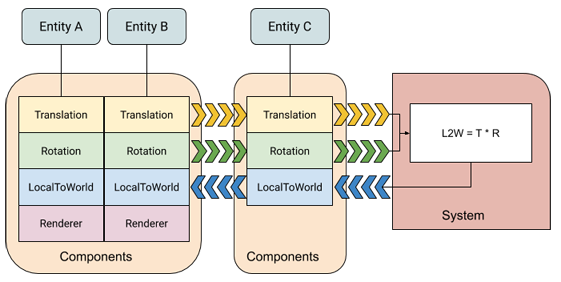
\includegraphics[scale=0.8]{Bilder/ECSConcept.png}
\caption{Zusammenspiel von \textit{Entities}, \textit{Components} und Systemen. Beispielhaft werden hier 3 \textit{Entities} gezeigt, wobei \textit{Entity} A und B fünf \textit{Components} haben und \textit{Entity} C nur vier \textit{Components} hat. \textit{Entity} C fehlt also das \texttt{Renderer} \textit{Component}. Das System nimmt als Eingabe alle \texttt{Translation} und \texttt{Rotation} \textit{Components} und modifiziert damit das \texttt{LocalToWorld} \textit{Component} der \textit{Entities}.}
\label{fig:ecs_concept}
\end{center}
\end{figure}
\subsubsection{\textit{Entities}\footnote{https://docs.unity3d.com/Packages/com.unity.entities@1.0/manual/concepts-entities.html}}\textit{Entities} repräsentieren meist Dinge in einem Unity Spiel. Das kann der Spielcharakter, Gegenstände, oder beliebige Gegner sein. Sie können aber auch abstrakte Dinge, wie beispielsweise Events repräsentieren. Ein Entity ist vergleichbar mit einem \textit{GameObject} im Objektorientierten in Unity. \textit{Entities} besitzen hierbei jedoch weder Daten noch ein Verhalten, sondern zeigen lediglich auf, welche Daten beziehungsweise \textit{Components} zueinander gehören. Alle \textit{Entities} in einer Spielwelt gehören zu einer sogenannten Welt\footnote{https://docs.unity3d.com/Packages/com.unity.entities@0.1/manual/world.html}. Zu dieser Welt gehört genau ein \textit{Entitymanager}\footnote{https://docs.unity3d.com/Packages/com.unity.entities@1.0/api/Unity.Entities.EntityManager.html}. Der \textit{Entitymanager} organisiert alle \textit{Entities} in dieser Welt. Mit ihm lassen sich \textit{Entities} erstellen, zerstören, \textit{Components} zu \textit{Entities} hinzufügen, entfernen oder verändern.
\subsubsection{\textit{Components}\footnote{https://docs.unity3d.com/Packages/com.unity.entities@1.0/manual/concepts-components.html}}
\textit{Components} repräsentieren die Daten des Spiels. \textit{Components} speichern die Daten eines \textit{Entity}. Diese Daten werden von Systemen genutzt und verarbeitet. Dabei unterscheidet man zwischen verwalteten \textit{Components} und unverwalteten \textit{Components}. Unverwaltete \textit{Components} werden in Unity als C\# Strukturen implementiert, sind leichtgewichtiger als Klassen. Diese können auch nur unverwaltete Daten speichern. Unverwaltete Daten sind beispielsweise Integer, Boolean, Bytes, Chars, oder andere Strukturen. Verwaltete \textit{Components} werden hingegen als Klassen definiert und können alle Daten halten. Es ist jedoch üblich unverwaltete \textit{Components} zu verwenden, da diese nicht so resourcenintensiv im Speichern und Zugriffen sind. Um ein unverwaltetes Component zu erstellen kann man das IComponentData Interface verwenden. Ein einfaches \textit{Component} könnte also wie folgt aussehen:
\begin{lstlisting}[style=code, caption={Beispiel unverwaltetes \textit{Component}}]
using Unity.Entities;
using Unity.Mathematics;

namespace ECS.Components
{
    public struct ExampleComponent : IComponentData
    {
        public int2 position;
        public float speed;
    }
}
\end{lstlisting}
Es gibt aber auch andere Arten von \textit{Components}. Es gibt \textit{Shared components}, \textit{Buffer components} und weitere\footnote{https://docs.unity3d.com/Packages/com.unity.entities@1.0/manual/components-type.html}. Es sind hier nicht alle \textit{Components} relevant, da manche lediglich die Spieleentwickelung mit dem datenorientierten Ansatz erleichtern, aber keine neue Funktion bieten. Zudem gibt es alle Arten von \textit{Components} sowohl als verwaltete als auch unverwaltete \textit{Components}.\\
\textbf{\textit{Shared Components}}: \textit{Shared Components} sind wie der Name schon sagt unter den \textit{Entities} gleich. Sie gruppieren die \textit{Entities} nach dem Wert des \textit{Shared Component}. \textit{Shared Components} werden abseits anderer \textit{Components} gespeichert und sind ein Weg um Datenduplizierung zu vermeiden. Unity speichert zusätzlich alle \textit{Entities}, welche die gleiche Kombination aus \textit{Component} Typen haben und das gleiche \textit{Shared Component} haben, also auch den gleichen Wert, gemeinsam. Dies hat zwar Vorteile, aber auch den großen Nachteil, dass das Ändern von Werten des \textit{Shared Component} ein verschieben der \textit{Entities} im Speicher zufolge hat. Die Probleme hierbei findet man in Kapitel \ref{structuralChanges}. Einen sehr großen und sinnvollen Vorteil haben \textit{Shared Components} in jedem Spiel das mit Unity's ECS entwickelt wird. Das RenderMesh \textit{Component}, also das \textit{Component} welches für das Aussehen der \textit{Entities} zuständig ist, ist immer ein \textit{Shared Component}. Dies ist sinnvoll, da sich diese \textit{Component} sehr selten im Wert ändert und viele \textit{Entities} das selbe RenderMesh \textit{Component} besitzen. Das kann ganz simpel einfach das Aussehen eines Baumes in einem Spiel sein. Oft gibt es viele Bäume in dem Spiel und diese ändern auch ihr Aussehen nicht.\\
\textbf{\textit{Buffer Components}}: Falls man mehrere \textit{Components} der selben Art auf einem \textit{Entity} haben möchte, sind \textit{Buffer Components} sehr hilfreich. Diese agieren wie ein Array von \textit{Components}. Zusätzlich sind \textit{Buffer Components} der Weg um ein Array an Daten zu speichern. Das ist besonder hilfreich, wenn man einem \textit{Entity} ein Inventar geben möchte, da dieses aus mehreren Gegenständen bestehen kann. Also kann man beispielsweise ein \textit{Buffer Component} für ein Inventar so entwerfen:
\begin{lstlisting}[style=code, caption={Buffer \textit{Component} Beispiel}]
using Unity.Entities;

namespace ECS.Components.Other
{
	//Array Kapazität auf acht festlegen
    [InternalBufferCapacity(8)]
    public struct ItemAmount : IBufferElementData
    {
        public int itemID;
        public int amount;
    }
}
\end{lstlisting}
Wie man sieht leitet die Struktur diesmal von IBufferElementData ab, welche den Typ \textit{Buffer Component} angibt. Zusätzlich wird hier das Attribut \textit{InternalBufferCapacity} genutzt. Damit legt man die Kapazität des \textit{Components} fest. Standardmäßig ist die Kapazität die Anzahl an Elementen, welche in 128 Bytes passen. Also hätten wir bei diesem Beispiel eine Kapazität von 16, da in einem \textit{Component} zwei Integer à 32 bit gespeichert werden. Jedoch braucht man für das Inventar beispielsweise nur 8 zu speichernde Gegenstände und kann so den benötigten Speicherplatz reduzieren.
\subsubsection{Systeme\footnote{https://docs.unity3d.com/Packages/com.unity.entities@1.0/manual/concepts-systems.html}}
Systeme beschreiben das Verhalten und beinhalten die Logik zum Transformieren der Daten. Die Systeme laufen ein mal pro ausgegebenem Bild mithilfe der \texttt{OnUpdate} Funktion auf dem \textit{main} Thread. Genau wie bei dem Objektorientierten von Unity gibt es auch hier mehrere Funktionen die zum Start / Ende ausgeführt werden. Zusätzlich kann man noch unter den definierten Systemen eine Reihenfolge festlegen, in der diese ausgeführt werden sollen. So wie bei den \textit{Components} gibt es auch bei den Systemen eine Klasse für verwaltete Daten (welche in diesem Fall von der Klasse SystemBase erbt) und eine Struktur für unverwaltete Daten (welche in diesem Fall das Interface ISystem implementiert). Zusätzlich sind Systeme immer an eine \textit{World} gebunden. Ein System für unverwaltete Daten und ohne implementierte Logik kann folgende Methoden implementieren:
\begin{lstlisting}[style=code, caption={System Beispiel}]
using Unity.Entities;

namespace ECS.Systems
{
    public partial struct ExampleSystem : ISystem, ISystemStartStop
    {
        //Wird beim Erstellen des Systems ausgeführt
        public void OnCreate(ref SystemState state){}
        //Wird vor dem ersten OnUpdate des Systems ausgeführt
        public void OnStartRunning(ref SystemState state){}
        //Wird für jedes ausgegebene Bild ausgeführt
        public void OnUpdate(ref SystemState state){}
        //Wird beim Stoppen des Systems ausgeführt
        public void OnStopRunning(ref SystemState state){}
        //Wird beim Zerstören des Systems ausgeführt
        public void OnDestroy(ref SystemState state){}
    }
}
\end{lstlisting}
Dabei ist das Interface ISystemStartStop optional und bietet die Möglichkeit bei dem Starten und Stoppen des Systems zusätzlich spezielle Logik auszuführen. Wie man sieht wird allen Funktionen auch eine Referenz des \textit{SystemState} übergeben. Darüber kann man auf verschiedene nützliche Dinge zugreifen, wie beispielsweise die \textit{World}, den \textit{EntityManager}, oder aber auch alle \textit{Components} eines Typs. Eine sinnvolle Herangehensweise ist es, in der \texttt{OnUpdate} Funktion Jobs zu schedulen. Dies wird in Kapitel \ref{jobs} weiter beschrieben.
\subsubsection{Archetypen\footnote{https://docs.unity3d.com/Packages/com.unity.entities@1.0/manual/concepts-archetypes.html}}
\begin{figure}[H]
\begin{center}
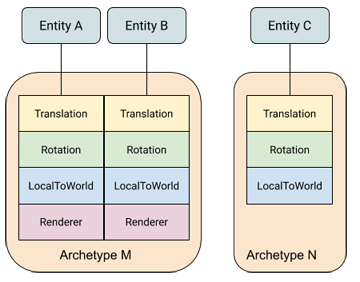
\includegraphics[scale=0.7]{Bilder/ArchetypeConcept.png}
\caption{Konzept von Archetypen. \textit{Entities}, welche die gleiche Zusammenstellung von \textit{Components} haben gehören einem Archetyp an. \textit{Entity} A und B gehören durch die gleiche Zusammenstellung an \textit{Components} also dem Archetyp M an und \textit{Entity} C hat eine andere Zusammenstellung Archetyp N an.}
\label{fig:archetype_concept}
\end{center}
\end{figure}
Ein Archetyp ist eine gewisse Zusammenstellung aus \textit{Components}. Jedes \textit{Entity} kann somit einem Archetyp zugeordnet werden. Beispielsweise sind alle \textit{Entities}, welche nur das ExampleComponent haben, einem Archetyp zugeordnet. \textit{Entities} welche zusätzlich \textit{Component} A besitzen gehören zu einem anderen Archetyp. Durch Archetypen ist es möglich, sehr performant, Datenorientiert zu arbeiten. Möchte man in einem System auf verschiedene \textit{Components} Operationen auszuführen, kann man alle Archetypen nach diesen \textit{Components} druchsuchen und muss nicht alle \textit{Entities} durchsuchen. Zusätzlich kann man diese Anfragen an Archetypen cachen um noch mehr Performance zu erreichen. Unity speichert alle \textit{Components} von \textit{Entities} für ein gewissen Archetyp in einem Block. Dieser wird auch \textit{Chunks} genannt. In Abbildung \ref{fig:archetyp_chunks} sieht man eine Visualisierung wie Archetypen mit \textit{Chunks} zusammenhängen:
\begin{figure}[H]
\begin{center}
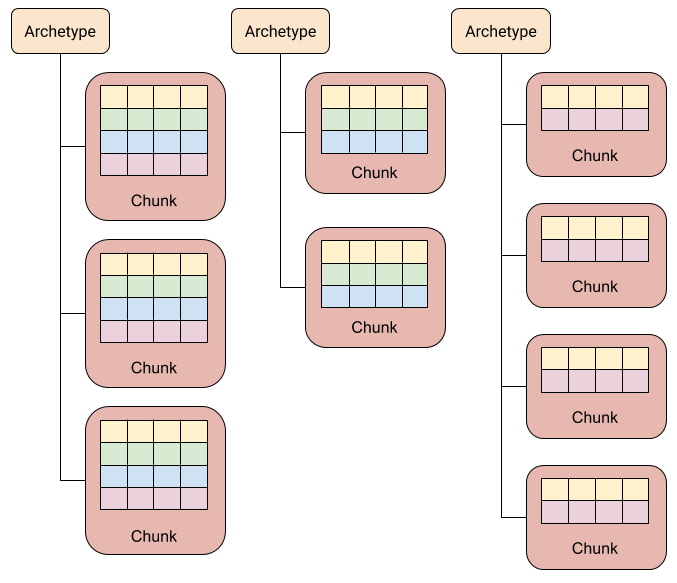
\includegraphics[scale=0.45]{Bilder/ArchetypeChunkDiagram.png}
\caption{Konzept von \textit{Chunks}. \textit{Chunks} sind Speicherbereiche für Archetypen. In dem Bild ist zu erkennen, dass der Archetyp links vier \textit{Components} hat (Anzahl an Reihen), der Archetyp in der Mitte drei \textit{Components} und der Archetyp rechts zwei \textit{Components}. In einen \textit{Chunk} passen hier jeweils vier \textit{Entities}, wobei dies von der Anzahl und Größe der jeweiligen \textit{Components} abhängig ist. Wenn ein \textit{Chunk} voll ist, muss ein neuer \textit{Chunk} erstellt werden. Daher kann es, abhängig von der Anzahl der \textit{Entities} in einem \textit{Chunk}, unterschiedlich viele \textit{Chunks} pro Archetyp geben.}
\label{fig:archetyp_chunks}
\end{center}
\end{figure}
Jeder dieser \textit{Chunks} ist 16 KiB groß. Demnach hängt es von den \textit{Components} ab, wie viele \textit{Entities} in einen \textit{Chunk} passen. Der \textit{Chunk} beinhaltet ein Array für jeden Typ der \textit{Components} und zusätzlich ein Array für die \textit{Entity} ID. Pro Arrayindex wird je ein \textit{Entity} gespeichert. Im Index 0 aller Arrays werden die Daten des ersten \textit{Entities} gespeichert. Falls ein \textit{Entity} zerstört, oder in einen anderen \textit{Chunk} bewegt wird (falls ein \textit{Component} hinzugefügt, oder entfernt wird), wird das letzte \textit{Entity} an seine Stelle bewegt. Falls ein \textit{Chunk} voll ist, erstellt der \textit{EntityManager} einen neuen falls eine \textit{Entity} hinzukommt. Leere \textit{Chunks} werden gelöscht.
\subsubsection{Strukturelle Änderungen}\label{structuralChanges}
Strukturelle Änderungen sind eines der wenigen unperformantem Themen in Unity's \textit{ECS}. Strukturelle Änderungen können das Erstellen und Zerstören eines \textit{Entities}, das Hinzufügen und Entfernen von \textit{Components}, oder das Ändern von Daten eines \textit{Shared Components} sein\footnote{https://docs.unity3d.com/Packages/com.unity.entities@1.0/manual/concepts-structural-changes.html}. Also im Grunde alles Operationen, welches das Ändern eines, oder mehrerer \textit{chunks} erfordert. Solche Änderungen könnten andere zur selben Zeit ausgeführten Aktionen invalidieren und müssen deshalb auf dem main Thread ausgeführt werden. Um dennoch Änderungen dynamisch an beliebiger Stelle ausführen zu können, nutzt man den \textit{Entity Command Buffer} (ECB). Mit dem ECB lassen sich strukturelle Änderungen sammeln und zu einem späteren Zeitpunkt in einer festgelegt Reihenfolge ausführen. So lassen sich problemlos aus einem Job strukturelle Änderungen sammeln und nach Beendigung des Jobs, diese auf dem main Thread ausführen. Das kann beispielsweise so aussehen:
\begin{lstlisting}[style=code, caption={ECB Beispiel}]
public void OnUpdate(ref SystemState state)
{
    //Neuer ECB wird erstellt
    EntityCommandBuffer ecb = new EntityCommandBuffer(Allocator.TempJob);
    //Job wird erstellt und der ECB wird übergeben
    new ExampleJob
    {
        ecb = ecb
    //Mit Schedule wird der Job gestartet
    }.Schedule();
    state.CompleteDependency();
    //Strukturelle Änderungen werden abgespielt
    ecb.Playback(state.EntityManager);
    //ECB muss auch wieder disposed werden
    ecb.Dispose();
}
\end{lstlisting}
Also erstellt man einen ECB, reiht verschiedene Aktionen in die Schlange ein und spielt diese auf dem main Thread wieder ab. Danach sollte man den ECB wieder disposen. Das gibt den Speicher für das Objekt wieder frei und räumt gegebenenfalls weitere Ressourcen auf. In dem Job kann man mit dem übergebenen ECB verschiedene Aktionen durchführen. Dies kann beispielsweise so aussehen:
\begin{lstlisting}[style=code, caption={ECB Aktionen Beispiel}]
//Ein Entity erstellen:
Entity newEntity = ecb.Instantiate(e);
//Dem Entity ein Component hinzufügen:
ecb.AddComponent<ExampleComponent>(newEntity);
\end{lstlisting}
Wie ein Job genau aussieht und funktioniert wird in Kapitel \ref{jobs} beschrieben.